\documentclass[12pt]{report}

\usepackage{graphicx}
\usepackage[spanish,mexico]{babel}
\usepackage[utf8]{inputenc}
\usepackage{amsmath}
\usepackage{fancyhdr}
\usepackage{float}
\usepackage{jslisting}
\usepackage{jslistings}

\graphicspath{ {./images/} }

\setlength{\oddsidemargin}{0in}
\setlength{\textwidth}{6in}
\setlength{\topmargin}{0in}
\setlength{\voffset}{0.5in}
\setlength{\hoffset}{0.5in}
% \setlength{\textheight}{8in}
\setlength{\textwidth}{5.5in}
\setlength{\topskip}{0in}
\setlength{\footskip}{1in}
\setlength{\parskip}{2ex}

\title{
   {“Diseño y desarrollo de sistema multi-plataforma para gestión de ventas y logística de microempresa.”}\\
   {\large INSTITUTO TECNOLÓGICO DE TIJUANA}\\
   {
\includegraphics{escudo1.png}}
}
\author{José Luis Murillo Ríos}
\date{21 DE JUNIO DEL 2019}


\begin{document}
\setcounter{page}{1}
\pagenumbering{roman}
\thispagestyle{empty}
\begin{center}
   INSTITUTO TECNOLÓGICO DE TIJUANA\\[0.75cm]
   Ingeniería en Sistemas Computacionales\\[0.8in]
\end{center}
\begin{figure}[h]
\begin{center}


\includegraphics[height=5.5 cm]{escudo1.png}
\vspace{0cm}
\end{center}
\end{figure}
\vspace{1cm}
\begin{center}
DISEÑO Y DESARROLLO DE SISTEMA MULTI-PLATAFORMA PARA GESTIÓN DE VENTAS Y LOGÍSTICA DE MICROEMPRESA.\\[4mm]
POR\\[4mm]
JOSÉ LUIS MURILLO RÍOS\\[1cm]
\small PARA OBTENER EL TÍTULO DE INGENIERO EN SISTEMAS COMPUTACIONALES
\vfill
TIJUANA, B.C. \hfill AGOSTO 2019
\end{center}

\newpage
\thispagestyle{empty}
\begin{center}
DISEÑO Y DESARROLLO DE SISTEMA MULTI-PLATAFORMA PARA GESTIÓN DE VENTAS Y LOGÍSTICA DE MICROEMPRESA.\\[1.3cm]
POR\\[0.8cm]
JOSÉ LUIS MURILLO RÍOS\\[0.8cm]
\small AGOSTO 2019\\[0.7cm]
\end{center}

% \chapter*{RESUMEN}
\newpage

\begin{center}
  {\Large \bf{RESUMEN}}
\end{center}
Cada día mas emprendedores inician su negocio con la ayuda de servcicios de venta en linea; muchas de estas empresas 
tienden a crecer y requerir de sistemas mas especializados que se ajusten a necesidades particulares.\\[0.8cm]
Se desarrolla un sistema que tiene como objetivo el llevar control de los procesos de venta y logística de una empresa.
El propósito del proyecto es integrar los servicios existentes de venta en linea de la compañía
y extender su uso, adaptándalos a los requerimientos específicas del cliente, así como diseñar una interfáz gráfica que permita
proporcionar un servicio mas rápido y agilice los proceso de elaboracion y entrega de productos.
 
% \chapter*{DEDICATORIA}
\newpage
\begin{center}
  {\Large  \bf{DEDICATORIA}}
\end{center}
\begin{center}
  A mis abuelos, por creer siempre en mi\\
  Gracias
\end{center}

 
% \chapter*{AGRADECIMIENTOS}
\newpage
\begin{center}
  {\Large  \bf{AGRADECIMIENTOS}}
\end{center}
\begin{center}
  Quiero dar gracias a Bolt Media por incluirme en su equipo y darme la oportunidad de crecer.
\end{center}


\newpage
\tableofcontents

\newpage
\listoftables
\addcontentsline{toc}{chapter}{Índice de Tablas} %%% Para introducir una línea en el índice
\listoffigures
\addcontentsline{toc}{chapter}{Índice de Figuras}
\lstlistoflistings

\chapter{Introducción}
\pagenumbering{arabic} %%% esto es para regresar el modo de numeración a numeración arábiga
\setcounter{page}{1}  %%% empezamos en página 1
\thispagestyle{empty}  %%%% la primera página no va enumerada

Muchas pequeñas empresas dependen en gran medida al éxito de sus ventas en linea, por lo que adoptan el uso de tecnologías robustas (como Shopify y WooCommerce) para su administración. su función principal es servir como puntos de entrada para los clientes pero dichos servicios no están diseñados para mostrar información detallada a distintas áreas de la empresa. Cada día mas emprendedores inician su negocio con la ayuda de estos servicios de venta en linea; algunos de estos negocios tienden a crecer y requerir de sistemas mas especializados que se ajusten a necesidades particulares.

\section{Antecedentes y definición del problema}
Se solicitó a la empresa Bolt Media Internacional S. de R.L. de C.V. desarrollar una plataforma que conectara las transacciones de rosesland.com, una plataforma de ventas en linea desarrollada en Shopify a las operaciones internas de la florería, como lo son las ventas de mostrador, la manufactura y la entrega de los productos.
\vspace{0.8cm}
Actualmente la florería realiza todo este proceso con comandas que los empleados de ventas llenan a mano, para después enviarlos al área de elaboración de arreglos florales y posteriormente se entregan al encargado de logística para dar indicaciones de la distribución de los productos. Este proceso de venta es lento y genera una experiencia poco placentera para los compradores, a su vez el área de manufactura está conformado por artesanos y trabajadores del campo que tienen un nivel de comprensión de lectura bajo y pueden llegar a cometer errores que retrasen todos los procesos. Por tales motivos este sistema debe ser fácil de usar para usuarios de distintas áreas y a su vez el diseño debe de adaptarse tanto a diferentes tamaños de pantallas como a diferentes dispositivos móviles. Se requiere una base de datos que notifique en tiempo real los cambios
en la información asi como un servidor que administre los permisos adecuados para su manipulación.

\section{Motivación para atender el problema}
Una de las herramientas mas poderosas para el comercio es el internet, 
saber aprovecharlo genera importantes beneficios para cualquier negocio, 
es por ello que la empresa Rosesland debe adoptar un proceso mas automatizado
en sus funciones y tomar ventaja de los ordenadores y dispositivos con los que cuenta la empresa.

\section{Propuesta de solución}
Implementar un sistema diseñado principalmente para ser utilizado en pantallas táctiles
que muestre las transacciones realizadas durante el día tanto en mostrador como en la pagina web,
dando un informe detallado de las operaciones de la compañia.

\section{Objetivos generales}
Automatizar el proceso de ventas y entregas de la floreía Rosesland 
e integrar los servicios de su tienda en linea rosesland.com 
mediante una aplicación web progresiva, que sea compatible con los dispositivos existentes de la empresa
y que funcione adecuadamente en navegadores de internet modernos.

\section{Objetivos específicos}
\begin{enumerate}
\item Desarrollar un servidor que adminstre la autenticación de los empleados y su acceso a la información.
\item Implementar una base de datos que notifique a los usuarios cambios en la información en tiempo real.
\item Diseñar una aplicacion web progesiva que garantice una experiencia de usuario óptima para todas las areas de la empresa
\item Integrar los servicios de la tienda en linea rosesland.com con las operaciones internas de la empresa, uniendo los procesos en una sola plataforma
\end{enumerate}


\chapter{Marco teórico}
\thispagestyle{fancy}
\pagenumbering{arabic} %%% esto es para regresar el modo de numeración a numeración arábiga
\setcounter{page}{1}  %%% empezamos en página 1
\thispagestyle{empty}  %%%% la primera página no va enumerada
Un \textbf{\textit{stack de aplicaciones}} es una colección de software o tecnologías que se utilizan para crear una aplicación web. Las aplicaciones de una sola página (SPA - Single Page Application) han crecido en popularidad ya que proporcionan una experiencia de usuario más fluida: llamadas de servidor livianas cambian lo que se muestra en la pantalla sin tener que actualizar toda la página. El resultado parece bastante ingenioso en comparación con la antigua forma de volver a cargar la página por completo. Esto provocó un aumento en los \textit{frameworks} de \textit{front-end}, ya que gran parte del trabajo se realizó en el lado del cliente. Aproximadamente al mismo tiempo, aunque completamente sin relación, las bases de datos NoSQL también comenzaron a ganar popularidad. El término \textit{stack} fue popularizado por primera vez por LAMP Stack: Linux, Apache, MySQL y PHP. Linux es el sistema operativo, Apache actúa como el servidor HTTP, MySQL proporciona la base de datos relacional para manejar la información de la aplicación y PHP es el lenguaje de programación en el que se construye la aplicación. MERN es un paquete de software que significa MongoDB, ExpressJS, ReactJS y NodeJS. Juntos, estos programas gratuitos mejoran la simplicidad del proceso de desarrollo web. Las opciones son muchas, pero elegir una puede ser difícil.

% \section{LAMP}
% LAMP es un acrónimo de Linux, Apache, MySQL, PHP (Perl o Python), componentes de código abierto. Funciona como un paquete de programas que proporcionan una plataforma robusta para desarrollar e implementar aplicaciones y servidores basados en web. Durante años, ha sido la solución más efectiva para desarrollar aplicaciones web de nivel empresarial con personalización y flexibilidad mejoradas, de manera rentable. LAMP sigue siendo relevante, es muy atractivo para muchos usuarios porque es asequible y eficiente, ofreciendo una excelente alternativa a los paquetes de software comerciales. 
\subsection{Componentes}
\begin{itemize}
  \item Linux (sistema operativo)
  \item Apache (servidor web)
  \item MySQL (persistencia de datos)
  \item PHP (lenguaje de programación)
\end{itemize}

Derivados:

\begin{itemize}
  \item LAMP (con Perl o Python en lugar de PHP)
  \item LAMP (con MongoDB en lugar de MySQL)
  \item WAMP (Windows como SO)
  \item MAMP (Mac OS X como SO)
  \item XAMPP (Cualquier servidor OS + Perl o PHP + FTP)
  \item LAPP (PostgreSQL como base de datos)
\end{itemize}

\subsection{Beneficios}
Es utilizado por cientos de miles de empresas y, por lo tanto, su mantenimiento está muy bien respaldado. Con infinitos módulos, bibliotecas y complementos disponibles, puede ser adaptado a las necesidades de una empresa.\\[0.8cm]
Es posible controlar el servidor y decidir qué versiones y software se instalarán, por lo que no tiene que depender del navegador del cliente.
\subsection{Desventajas}
Debido a que es fácil de aprender, es posible caer en malas prácticas y crear aplicaciones basura. Comenzar con PHP, Python o Perl es fácil, pero dominarlo es difícil. Esto también es cierto para la seguridad en estas aplicaciones.

\section{MEAN/MERN}
En comparación con LAMP, el paquete de aplicaciones MEAN es bastante nuevo. Una de sus mayores diferencias es que MEAN no depende de un sistema operativo específico. Node.js se encarga de la ejecución del lado del servidor. MEAN Stack se recomienda especialmente para desarrolladores de JavaScript, ya que utiliza JavaScript en todos los niveles, tanto para el código del lado del cliente, así como el código del lado del servidor. Angular, el potente \textit{framework} de \textit{front-end}, utiliza un patrón de diseño Modelo-Vista-Controlador. A medida que React crece en popularidad, ha presentado una opción alternativa para el desarrollo \textit{frontend}, aunque React es simplemente una biblioteca, no un \textit{framework} MVC completo. MongoDB es un juega un papel importante y una opción increíblemente popular en el mundo de la gestión de bases de datos NoSQL. Node.js le permite al programador escribir el back-end de la aplicación en Javascript, Express.js se usa encima de Node para manejar las solicitudes de enrutamiento y proporcionar una API REST, o incluso puede usarse para generar el HTML final para ser utilizado por el \textit{framework} de \textit{front-end}.
\subsection{Componentes}
\begin{itemize}
  \item MongoDB (base de datos)
  \item Express.js (servidor)
  \item Angular.js (cliente)
  \item Node.js (entorno del servidor)
\end{itemize}

Derivados:

\begin{itemize}
  \item MERN (React.js en lugar de Angular.js)
  \item MEEN (Ember.js en lugar de Angular.js)
\end{itemize}

\begin{figure}[H]
  \centering
  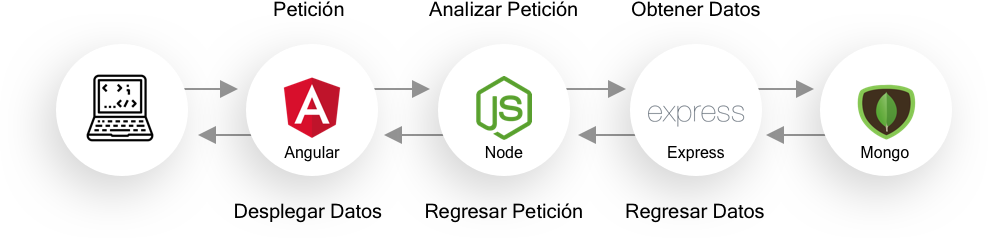
\includegraphics[width=1\textwidth]{mean}
  \caption{Flujo de informacion en MEAN Stack.}
\end{figure}

\subsection{Base de datos NOSQL}
Las bases de datos NOSQL son una alternativa emergente a las bases de datos relacionales más utilizadas. Como su nombre lo indica, no reemplaza completamente a SQL, sino que lo complementa de tal manera que puedan coexistir \\[0.8cm]
El concepto de NOSQL se desarrolló hace mucho tiempo, pero fue después de la introducción de la base de datos como servicio (DBaaS) que obtuvo un reconocimiento destacado. Debido a la alta escalabilidad proporcionada por NOSQL, fue visto como un importante competidor del modelo de base de datos relacional. A diferencia de RDBMS, las bases de datos NOSQL están diseñadas para escalar fácilmente a medida que crecen. La mayoría de los sistemas NOSQL han eliminado el soporte multiplataforma y algunas características adicionales innecesarias de RDBMS, haciéndolos mucho más livianos y eficientes que sus contrapartes RDMS.
\subsection{Orientado a documentos}
El concepto principal de una base de datos orientada a documentos es que el documento contiene grandes cantidades de datos que pueden estar disponibles de manera útil. Se puede acceder a estos documentos como un directorio regular en el que puede tener diferentes colecciones y cada colección tiene documentos que contienen la información deseada. Además, cada colección puede tener colecciones internas. Puede tener un árbol completo de documentos, sin embargo, esta práctica no se recomienda y debe evitar tener más de tres niveles de anidamiento. \\[0.8cm]
Las bases de datos NoSQL no son necesariamente bases de datos relacionales. Los datos no son representados en términos de filas y columnas de tablas. En MongoDB, los datos se visualizan como objetos o documentos. Esto ayuda a un programador a evitar una capa de traducción, por lo que no es necesario convertir o asignar los objetos con los que trata el código en tablas relacionales. Dichas traducciones se denominan capas de Mapeo Relacional de Objetos (ORM).
\begin{figure}[H]
  \centering
  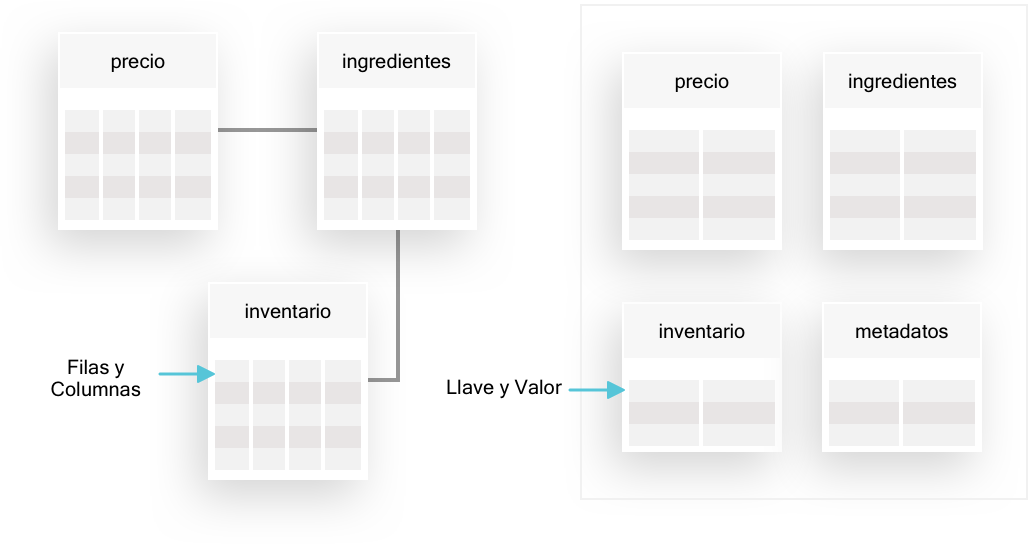
\includegraphics[width=1\textwidth]{sql-nosql}
  \caption{Diagrama que representa las diferencias clave entre la base de datos SQL y las bases de datos NoSQL.}
\end{figure}
\subsection{Angular/React}
Angular o React, proporcionan la interfaz de usuario reactiva de su aplicación. Utilizan componentes, son reactivos porque el usuario recibe cambios inmediatos cuando interactúa con la aplicación y, por lo general, se ejecutan dentro del navegador de un usuario (aunque ambos son isomórficos, capaces de ejecutarse en un servidor). \\[0.8cm]
\subsection{Beneficios}
Usar JavaScript como el lenguaje de programación principal es una gran ventaja. Todo se puede configurar rápidamente y hacer en JavaScript, lo que hace que sea mucho más fácil encontrar desarrolladores, y los desarrolladores de LAMP generalmente también conocen JavaScript. Otra gran ventaja es la capacidad de crear fácilmente aplicaciones móviles o de escritorio, por ejemplo con Ionic. El código y los componentes se pueden reutilizar o agregar fácilmente.
\subsection{Desventajas}
Muchas librerías y \textit{frameworks} son bastante nuevos, y las nuevas versiones se lanzan rápidamente, por lo que mantener una aplicación puede ser una molestia. Dado que muchas tecnologías desaparecen después de unos años, la sostenibilidad puede convertirse en un problema. También es más difícil mantener una base de código limpia y seguir las mejores prácticas a medida que su aplicación crece. Además, debe confiar en el cliente y las tecnologías disponibles del cliente.

\newpage
\section{FERN}
Firebase es una plataforma propiedad de Google que tiene como objetivo proporcionar un enfoque holístico para un rápido desarrollo web y móvil. En resumen, le permite centrarse en las partes frontales de la aplicación. Se completa con una base de datos visual sin tablas (NoSQL), alojamiento, almacenamiento de archivos, procesamiento del lado del servidor para cosas que deben protegerse de la interfaz y un sistema de autenticación, todo lo necesario para aplicaciones pequeñas y medianas. \\[0.8cm]
% \subsection{Servicios de Firebase}
% \begin{itemize}
%   \item Base de datos
%   \item Autenticación
%   \item Almacenamiento
%   \item Notificaciones
%   \item Análisis
% \end{itemize}
Cloud Firestore es el servicio de base de datos de Google Firebase para aplicaciones móviles. Firestore permite una experiencia de programación increíble cuando se usa en un stack de aplicaciónes completo. Los datos en tiempo real y la facilidad de conexión a la base de datos hacen que la pila FERN sea una forma rápida de conectar estas tecnologías. 
\subsection{Componentes}
\begin{itemize}
  \item Firebase (base de datos)
  \item Express.js (servidor)
  \item React.js (cliente)
  \item Node.js (entorno del servidor)
\end{itemize}
\begin{figure}[H]
  \centering
  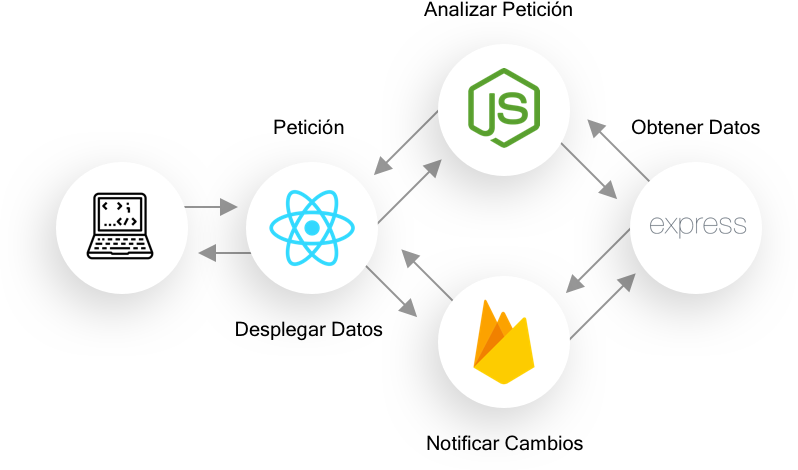
\includegraphics[width=0.8\textwidth]{fern}
  \caption{Flujo de informacion en FERN Stack.}
\end{figure}
\subsection{Cloud Firestore}
Firestore es una bases de datos orientada a documentos, toda la información se guarda en colecciones como JSON, principalmente diseñada para almacenar, recuperar y administrar información orientada a documentos, también conocida como datos semiestructurados.\\[0.8cm]
La escalabilidad es completamente automática, lo que significa que no es necesario compartir sus datos en varias instancias. Los cargos de Cloud Firestore se basan en las operaciones realizadas en su base de datos (lectura, escritura, borrado), ancho de banda y almacenamiento. Admite límites de gasto diario para proyectos de Google App Engine, para garantizar que no exceda los costos con los que el usuario se sienta cómodo.
\begin{figure}[H]
  \centering
  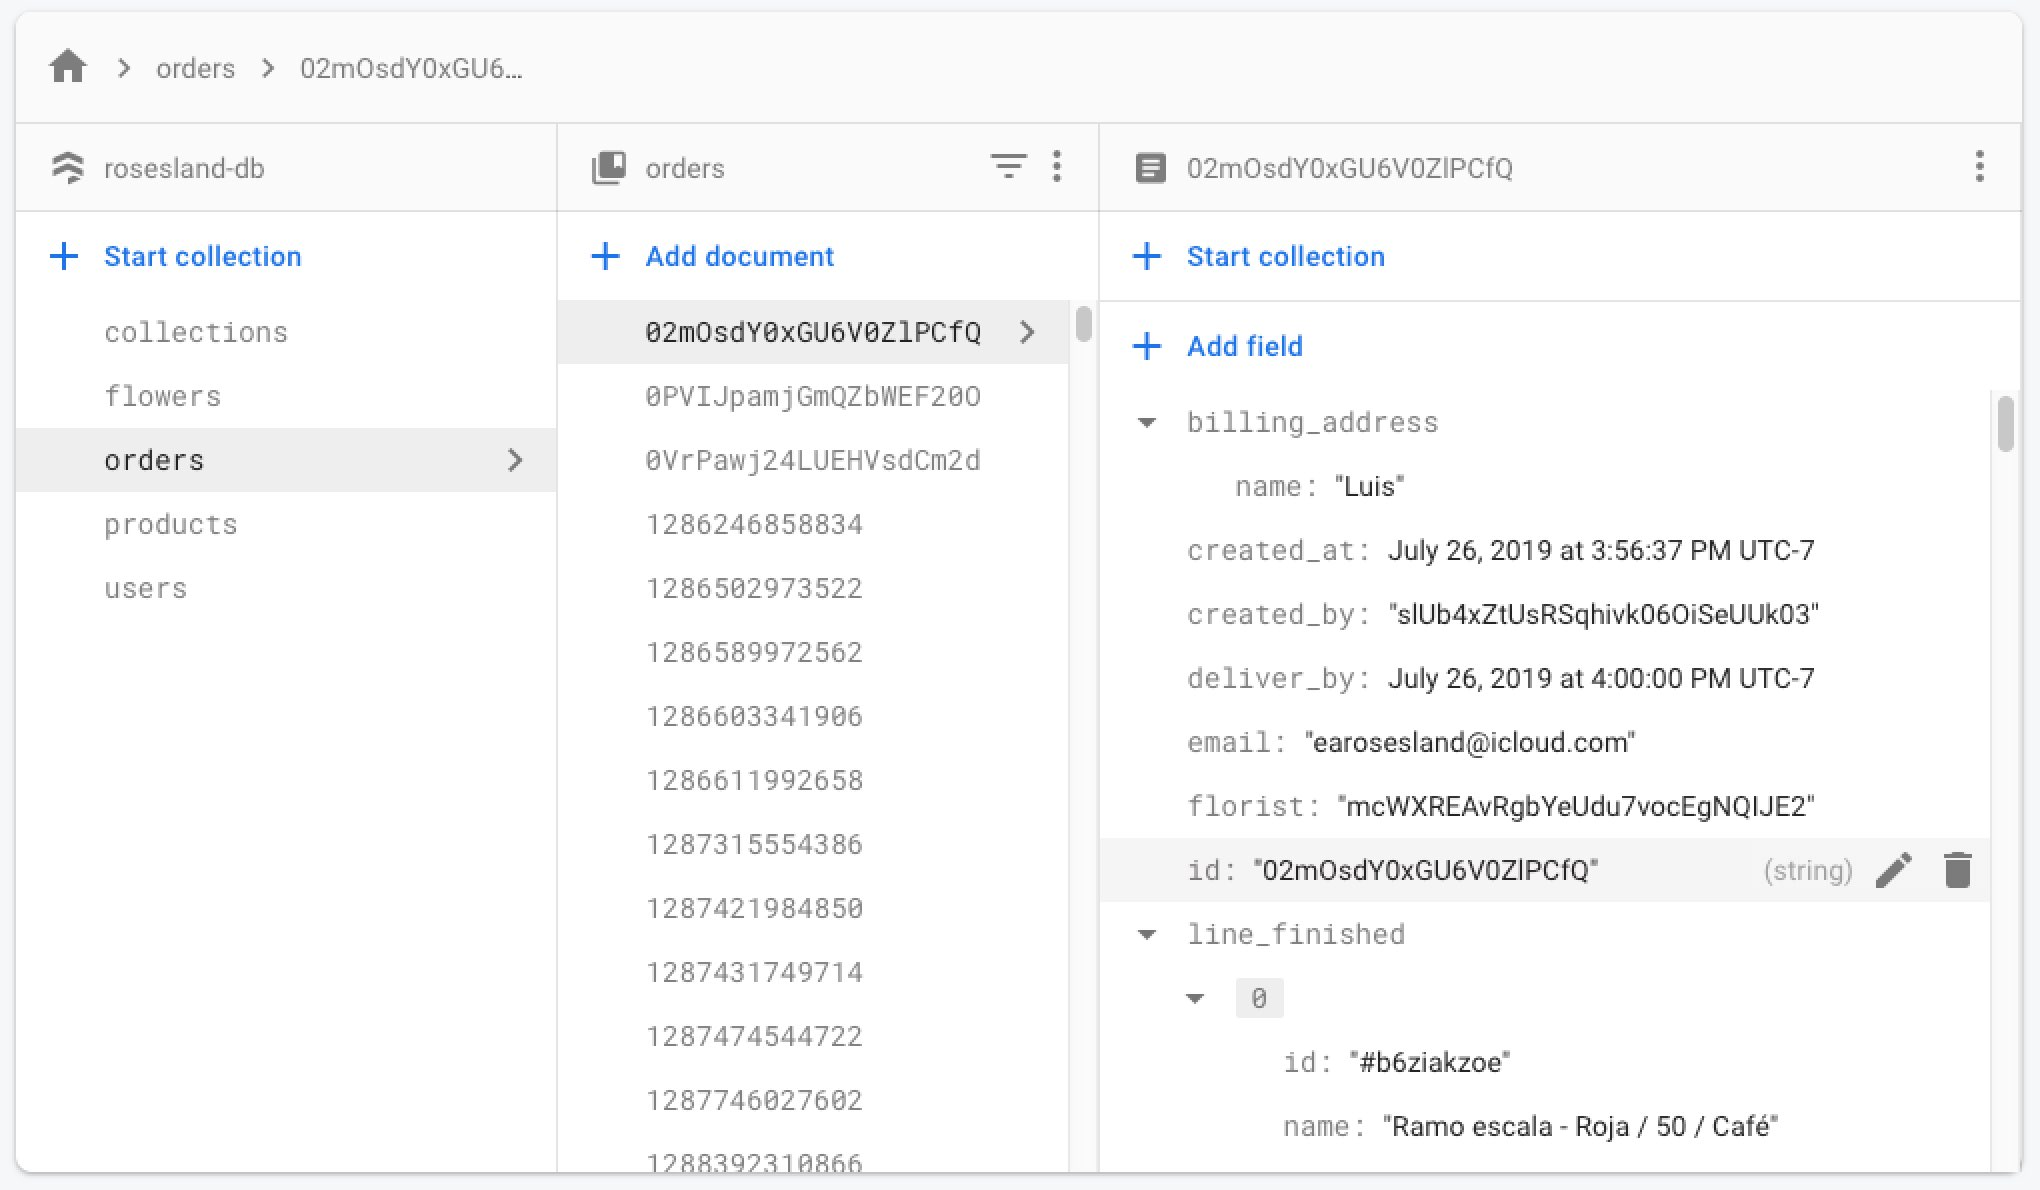
\includegraphics[width=0.9\textwidth]{firestore}
  \caption{Colección de Firestore con sus documentos internos.}
\end{figure}
\subsection{Node.js}
Node.js es un entorno multiplataforma de código abierto para ejecutar código JavaScript del lado del servidor. El entorno de tiempo de ejecución de Node.js incluye todo lo que necesita para ejecutar un programa escrito en JavaScript. \\[0.8cm]
Node.js surgió cuando los desarrolladores originales de JavaScript lo extendieron de algo que solo podía ejecutar en el navegador a algo que podría ejecutar en su máquina como una aplicación independiente. Ahora puede hacer mucho más con JavaScript que simplemente hacer que los sitios web sean interactivos. JavaScript ahora tiene la capacidad de hacer cosas que otros lenguajes de secuencias de comandos como Python pueden hacer. Tanto su navegador JavaScript como Node.js se ejecutan en el motor de tiempo de ejecución JavaScript V8. Este motor toma su código JavaScript y lo convierte en un código de máquina más rápido. El código de máquina es un código de bajo nivel que la computadora puede ejecutar sin necesidad de interpretarlo primero.
\begin{figure}[H]
  \centering
  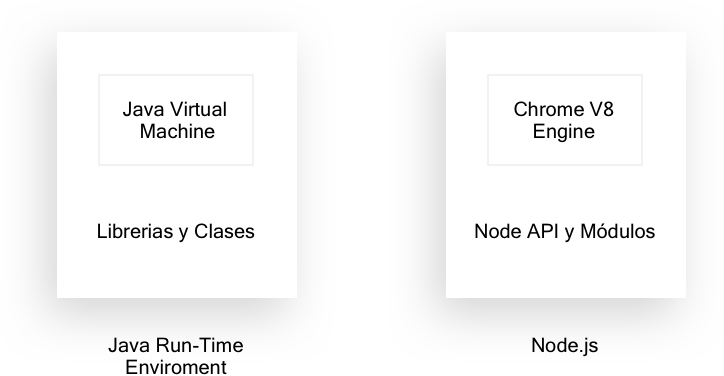
\includegraphics[width=0.8\textwidth]{node}
  \caption{Analogía Node.js con Java.}
\end{figure}
\subsubsection{Motor V8 de Google Chrome}
Node.js utiliza el motor de ejecución ultra rápido V8 de Google Chrome. Hasta el lanzamiento de Chrome, la mayoría de los navegadores leían JavaScript de manera ineficiente: el código se leía e interpretaba poco a poco. Tomó mucho tiempo leer JavaScript y convertirlo a lenguaje máquina para que el procesador pudiera entenderlo. \\[0.8cm]
El motor V8 de Google Chrome funciona completamente diferente. Está altamente optimizado y lleva a cabo lo que llamamos compilación JIT (Just In Time). Transforma rápidamente el código JavaScript en lenguaje máquina.
% \subsubsection{Características}
% \begin{itemize}
  %   \item Node.js utiliza un modelo de E/S (I/O) sin bloqueo controlado por eventos que lo hace ligero y eficiente.
  
  %   \item El ecosistema de paquetes de Node.js, \textit{npm}, es el ecosistema de bibliotecas de código abierto más grande del mundo.
% \end{itemize}
\subsection{El ecosistema NPM}
NPM (Node Package Manager) es el administrador de paquetes predeterminado para Node.js. se instala en el sistema con la instalación de Node.js. Los paquetes y módulos necesarios en un proyecto Node se instalan utilizando \textit{npm}.\\[0.8cm]
NPM consta de tres componentes:
\begin{enumerate}
  \item Sitio web
  \item Registro
  \item CLI
\end{enumerate}
\subsubsection{Sitio web}
El sitio web oficial de npm es https://www.npmjs.com/. Con este sitio web puede encontrar paquetes, ver documentación, compartir y publicar paquetes.
\subsubsection{Registro}
El registro npm es una gran base de datos que consta de más de medio millón de paquetes. Los desarrolladores descargan paquetes del registro npm y publican sus paquetes en el registro.
\subsubsection{CLI (interfaz de línea de comando)}
Esta es la línea de comando que ayuda a interactuar con el npm para instalar, actualizar y desinstalar paquetes y administrar dependencias.
\subsection{Comandos NPM}
Npm tiene muchos paquetes que puedes usar en una aplicación para que su desarrollo sea más rápido y eficiente. Instalar módulos usando NPM no representa un gran problema. Hay una sintaxis simple para instalar cualquier módulo Node.js:
\begin{verbatim}
  npm install <Nombre del módulo>
  ejemplo:
  npm install express
\end{verbatim}
\subsection{Express.js}
Escribir un servidor web completo a mano en Node.js directamente no es tan fácil, ni es necesario, Express.js es un paquete de aplicación web minimalista y extensible creado para el ecosistema Node.js. Permite crear un servidor web legible, flexible y fácil de mantener. \\[0.8cm]
Express.js le permite definir rutas, especificaciones de qué hacer cuando llega una solicitud HTTP que coincide con un patrón determinado. La especificación coincidente se basa en expresiones regulares (regex) y es muy flexible, como la mayoría de los otros entornos de aplicaciones web. La parte de qué hacer es solo una función que recibe la solicitud HTTP analizada. \\[0.8cm]
Express.js analiza la URL de solicitud, encabezados y parámetros. En el lado de la respuesta, tiene, como se esperaba, toda la funcionalidad requerida por las aplicaciones web. Esto incluye la configuración de códigos de respuesta, configuración de cookies, envío de encabezados personalizados, etc. Además, puede escribir middleware Express, piezas de código personalizadas que se pueden insertar en cualquier ruta de procesamiento de solicitud/respuesta para lograr una funcionalidad común como el registro, la autenticación, entre otras.
\subsection{React.js}
React es una biblioteca de JavaScript declarativa, eficiente y flexible creada en 2013 por el equipo de desarrollo de Facebook. React quería que las interfaces de usuario fueran más modulares (o reutilizables) y más fáciles de mantener. Según el sitio web de React, se utiliza para \textit{construir componentes encapsulados que administran su propio estado, y unirlos para crear interfaces de usuario complejas}. React es una biblioteca JavaScript que permite componer interfaces de usuario complejas a partir de piezas de código pequeñas y aisladas llamadas \textit{componentes}.
\subsection{Componentes}
Un componente es una pequeña parte de la interfaz de usuario. Todas las piezas reutilizables de una página web se abstraen en un componente.
\begin{figure}[H]
  \centering
  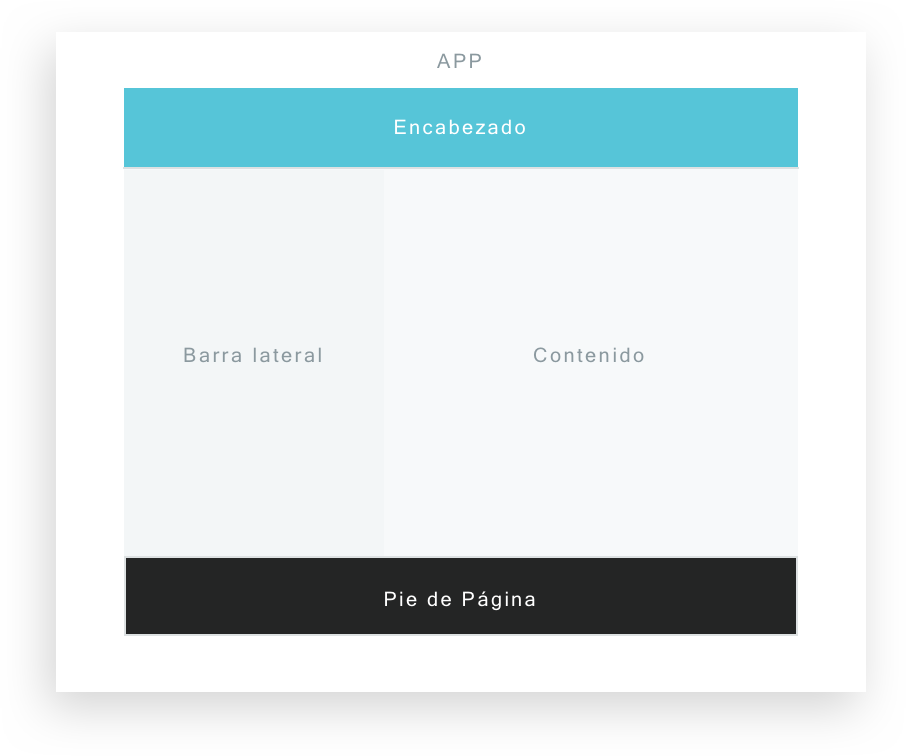
\includegraphics[width=0.8\textwidth]{components}
  \caption{Componentes principales de una página web.}
\end{figure}
En primer lugar, hay un componente principal llamado componente APP. Este componente de la aplicación contiene cuatro componentes secundarios o se divide en cuatro componentes:
\begin{enumerate}
  \item Encabezado
  \item Barra lateral
  \item Contenido
  \item Pie de página
\end{enumerate}
La función de cada componente se manejará independientemente con otros componentes. Cada componente es una pieza reutilizable, y se puede pensar en cada componente de forma aislada. \\[0.8cm]
Dentro de un componente, tendremos subcomponentes o componentes dentro de un componente padre. Esos serán reutilizables también.
\subsection{DOM Virtual}
React utiliza algo llamado DOM virtual, que es una representación virtual del DOM. Detrás de escena, React hace un gran trabajo para editar y volver a renderizar eficientemente el DOM cuando algo en la interfaz necesita cambiar.

\newpage
\section{Preprocesamiento}
\subsection{ES5/ES6}
ES5 (ES significa ECMAScript) es básicamente `JavaScript normal'. La quinta actualización de JavaScript, ES5 se finalizó en 2009. Ha sido compatible con todos los principales navegadores durante muchos años. \\[0.8cm]
ES6 es una nueva versión de JavaScript que agrega algunas buenas adiciones sintácticas y funcionales. Se finalizó en 2015. ES6 es casi totalmente compatible con todos los navegadores principales. Pero pasará algún tiempo hasta que las versiones anteriores de los navegadores web estén fuera de uso. Por ejemplo, Internet Eyplorer 11 no es compatible con ES6, pero tiene aproximadamente el 8\% de uso de mercado de navegadores.\\[0.8cm]
Para aprovechar los beneficios de ES6 hoy, se tienen que hacer que hacer algunos procedimientos para que funcione en tantos exploradores de internet como sea posible:
\begin{enumerate}
  \item Se debe preprocesar el código para que una gama más amplia de navegadores entiendan nuestro JavaScript. Esto significa convertir ES6 JavaScript en ES5 JavaScript.
  \item Tenemos que incluir un `shim' o `polyfill' que brinde una funcionalidad adicional agregada en ES6 que un navegador puede o no tener.
\end{enumerate}
\subsubsection{JSX}
JSX es una extensión de sintaxis similar a XML para ECMAScript sin ninguna semántica definida. NO está destinado a ser implementado por motores o navegadores. NO es una propuesta para incorporar JSX en la propia especificación ECMAScript. Está destinado a ser utilizado por varios preprocesadores (transpiladores) para transformar estos tokens en ECMAScript estándar.
\subsubsection{BabelJS}
BabelJS es un transpilador de JavaScript que transpila nuevas características ES6 al antiguo estándar ES5. Con esto, las funciones se pueden ejecutar en navegadores antiguos y nuevos, sin problemas. \\[0.8cm]
\textbf{El preprocesador BabelJS} convierte la sintaxis de JavaScript moderno en un formulario, que los navegadores más antiguos pueden entender fácilmente. Por ejemplo, const y let se convertirán en var, la función flecha se convierte en una función normal manteniendo la funcionalidad igual en ambos casos.
\subsubsection{Sass (Syntactically Awesome Style Sheets)}
Sass es un preprocesador de CSS, que ayuda a reducir la repetición con CSS y ahorra tiempo. Es un lenguaje de extensión CSS más estable y potente que describe el estilo de una página estructuralmente. Sus principales atributos son:
\begin{enumerate}
  \item Es un súper conjunto de CSS, lo que significa que contiene todas las características de CSS y es un preprocesador de código abierto, codificado en Ruby.
  \item Proporciona algunas características, que se utilizan para crear hojas de estilo que permiten escribir código más eficiente y fácil de mantener.
\end{enumerate}
\subsubsection{Webpack}
Webpack es un empaquetador de módulos. Webpack toma un archivo de entrada, encuentra todos los archivos de los que depende y genera un archivo que contiene todo el código de una aplicación. Con él es posible importar archivos CSS e imágenes directamente a JavaScript. Se puede compilar CoffeeScript, TypeScript, SASS y LESS. También es capaz de compilar la sintaxis de ES6 en JavaScript amigable para el navegador. En otras palabras, Webpack toma diferentes archivos (como CSS, JS, SASS, JPG, SVG, PNG, etc.) y los combina en paquetes, un paquete separado para cada tipo de archivo.

\newpage
\section{Control de versiones}
Hoy en día no es prudente empezar un proyecto web sin una estrategia de respaldo. Debido a que los datos son efímeros y se pueden perder fácilmente, por ejemplo, a través de un cambio de código erróneo o un fallo catastrófico de disco, es aconsejable mantener un archivo de todo el trabajo.\\[0.8cm]
Para proyectos de texto y código, la estrategia de respaldo generalmente incluye control de versiones, o seguimiento y administración de revisiones.  Dado su papel fundamental, el control de versiones es más efectivo cuando se adapta a los hábitos y objetivos de trabajo del equipo del proyecto.\\[0.8cm]
En su forma más simple, un sistema de control de versiones proporciona un principio básico y un método para almacenar archivos y cambios realizados en ellos. Esto se logra mediante el uso de un repositorio. El repositorio contiene la versión más reciente de cada archivo y el historial de cambios que ha llevado a esa representación. Por lo general, cada cambio incluye información adicional, como el autor y una breve descripción.
\subsection{Git}
Git es un software de control de versiones distribuido particularmente potente, flexible y de bajo costo que hace que el desarrollo colaborativo sea un placer. \\[0.8cm]
La principal diferencia entre Git y cualquier otro versionador es la forma en que Git piensa acerca de sus datos. Conceptualmente, la mayoría de los otros sistemas almacenan información como una lista de cambios basados en archivos. Estos sistemas (CVS, Subversion, Perforce, Bazaar, etc.) piensan en la información que mantienen como un conjunto de archivos y los cambios realizados en cada archivo a lo largo del tiempo. Git no piensa ni almacena sus datos de esta manera. En cambio, Git piensa en sus datos más como un conjunto de instantáneas de un mini sistema de archivos. Cada vez que confirma o guarda el estado de su proyecto en Git, básicamente toma una fotografía de cómo se ven todos sus archivos en ese momento y almacena una referencia a esa instantánea. Para ser eficiente, si los archivos no han cambiado, Git no almacena el archivo nuevamente, solo un enlace al archivo idéntico anterior que ya ha almacenado. \\[0.8cm]
\begin{figure}[H]
  \centering
  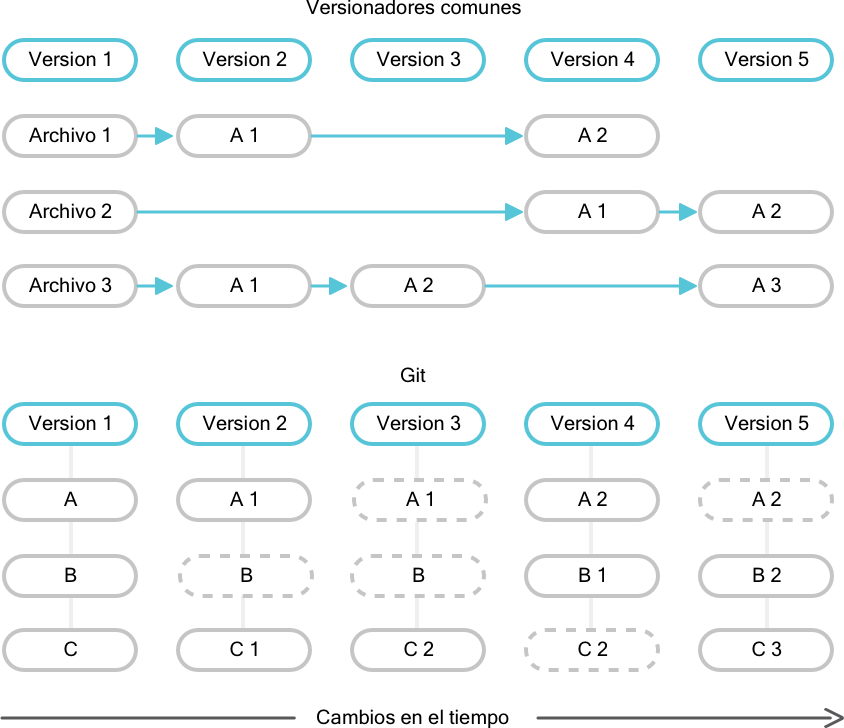
\includegraphics[width=0.9\textwidth]{git}
  \caption{Diferencias entre controladores de versiones. (Fuente: Elaboración propia)}
\end{figure}


\chapter{Análisis y diseño del sistema}
Las microempresas constituyen una potencia impulsora y se consideran entre las principales fuentes de trabajo, no obstante, es muy común encontrar microempresas con dificultades de crecimiento, principalmente debido a una mala administración o por falta de aprovechamiento de sus recursos. \\[0.8cm]
A continuación se describen los procedimientos necesarios para elaborar un sistema que permita a la empresa Rosesland llevar control de las ventas, elaboración y entrega de productos, así como incorporar los servicios de su tienda en linea al sistema. Permitiendo a la empresa tomar ventaja de las tecnologías web mas recientes, aprovechando al máximo los recursos existentes de la compañia.

\section{E-Commerce (Comercio electrónico)}
El comercio electrónico se refiere al proceso de compra o venta de productos o servicios a través de Internet. Las compras en línea se están volviendo cada vez más populares debido a la velocidad y facilidad de uso para los clientes. Las actividades de comercio electrónico, como la venta en línea, pueden dirigirse a consumidores u otras empresas. Vender en línea puede ayudar a su empresa a llegar a nuevos mercados y aumentar sus ventas e ingresos (ya sea a través de su propio sitio web o de un sitio de mercado electrónico).

\begin{figure}[H]
  \centering
  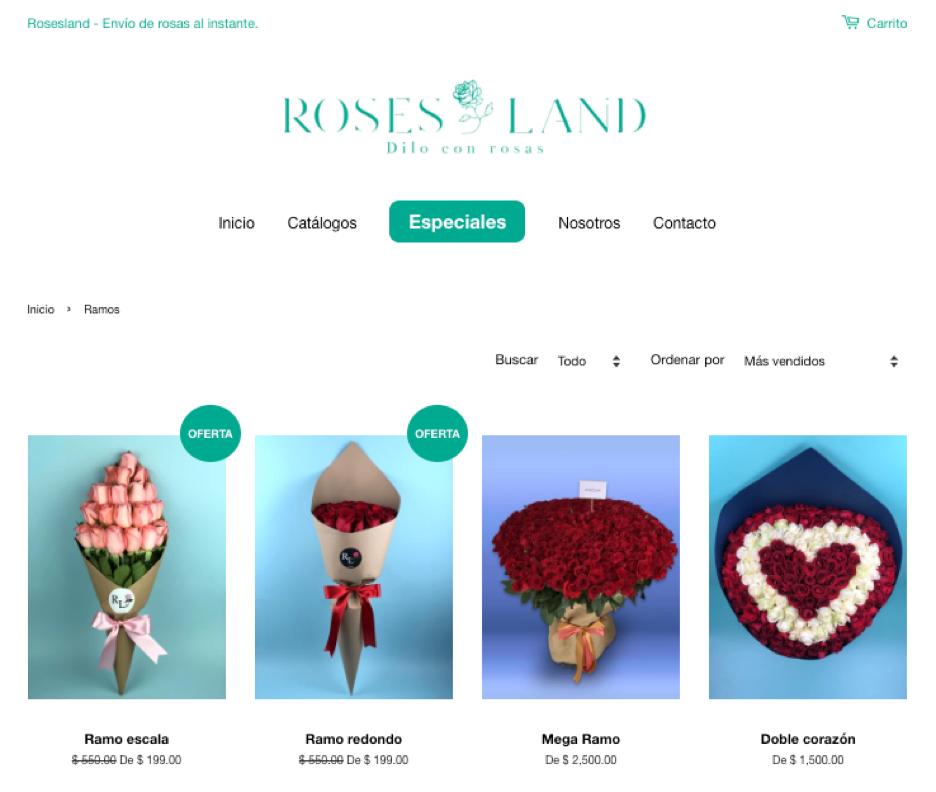
\includegraphics[width=0.9\textwidth]{rosesland}
  \caption{Tienda en linea actual de la empresa.}
\end{figure}

\subsubsection{Shopify}
Shopify es un servicio web que le permite configurar una tienda en línea para vender sus productos. 
Le da la facilidad organizar sus productos, personalizar el diseño de su tienda, 
aceptar pagos con tarjeta de crédito, rastrear y responder a pedidos. 
Shopify.com permite a los vendedores elegir entre opciones de diseño gratuitas 
o diseños personalizados creados por los usuarios.

\begin{figure}[H]
  \centering
  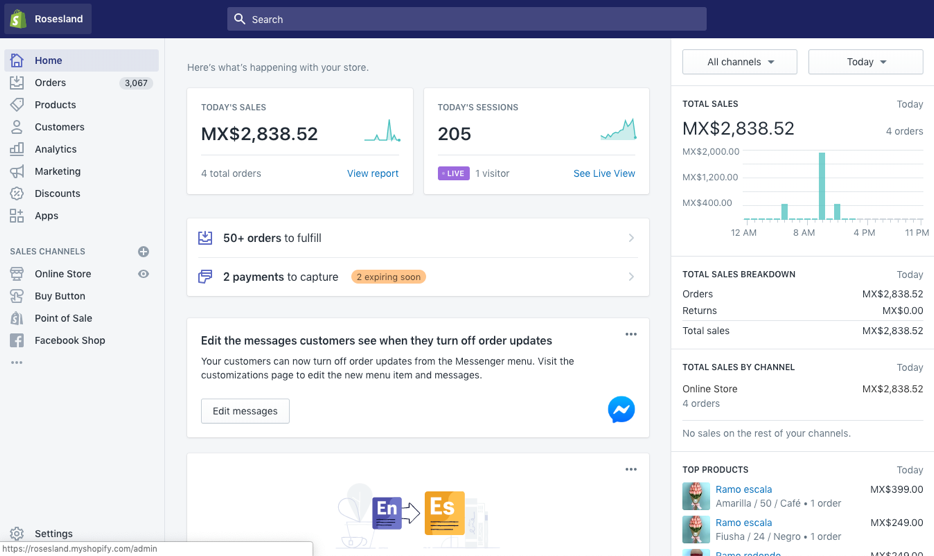
\includegraphics[width=0.9\textwidth]{shopify}
  \caption{Interfaz del administrador Shopify.}
\end{figure}

\section{Requerimientos del proyecto}
El producto final está enfocado en incrementar las ventas de la empresa Rosesland, con la ayuda de una plataforma que administre y mejore sus procesos internos. La finalidad del proyecto es disminuir los tiempos de ventas, elaboración y entrega de productos, así como la de crear un vínculo entre el servidor y su infraestructura actual extendiendo sus capacidades.
\vspace{0.8cm}

El sistema debe adaptarse al sistema operativo Linux. Anticipado a futuros cambios en la plataforma se decide trabajar con Node.js, ya que es de código abierto y multiplataforma, esto permite beneficiarse de la reutilización del código y la falta de cambio de contexto. Las aplicaciones Node.js están escritas en JavaScript puro y pueden ejecutarse dentro del entorno Node.js en Windows, Linux, etc.
\vspace{0.8cm}

La interfaz gráfica de usuario de la aplicación debe ser responsiva y funcionar en la mayoría de los navegadores web modernos, además debe ser fácil de aprender, idealmente requerir poco entrenamiento.
\vspace{0.8cm}

\subsection{Herramientas}
Node.js permite incorporar herramientas poderosas a proyectos de cualquier tipo. Esto incluye todo, desde bibliotecas y \glspl{framework} como jQuery y AngularJS hasta procesadores de código como Webpack. Los paquetes vendrán en una carpeta típicamente llamada node\_modules, que también contendrá un archivo package.json. Este archivo contiene información sobre todos los paquetes, incluidas las dependencias, que son módulos adicionales necesarios para usar un paquete en particular.

\subsubsection{Dependencias de desarrollo}
Las dependencias de desarrollo son aquellas que se utilizan dentro del entorno de programación. Aquí se incluyen herramientas que no forman parte del ejecutable final como lo son lo preprocesadores, empaquetadores y analistas de código. Los principales módulos de desarrollo son los siguientes:
\begin{itemize}
  \item Babel: es un compilador de JavaScript utilizado para convertir código ECMAScript 2015+ (ES6+) en una versión que pueda ser ejecutado en motores JavaScript más antiguos.
  \item Webpack: es un empaquetador de módulos principalmente para JavaScript, pero puede transformar archivos \gls{frontend} como HTML, CSS e imágenes si se incluyen los complementos correspondientes.
  \item ESLint: es una herramienta de análisis de código estático para identificar patrones problemáticos encontrados en el código JavaScript.
  \item PostCSS: es una herramienta de desarrollo de software que utiliza complementos basados en JavaScript para automatizar las operaciones de rutina de CSS. Con este modulo es posible analizar CSS, agregar prefijos de proveedor a las reglas CSS, ejecutar optimizaciones enfocadas, para garantizar que el resultado final sea lo más pequeño posible para un entorno de producción.
  \item Pug: es un preprocesador que simplifica la tarea de escribir HTML. También agrega funcionalidades, como objetos Javascript, condiciones, bucles, \glspl{mixin} y plantillas.
\end{itemize}

\subsubsection{Estructura del proyecto}
La estructura del proyecto Node.js está influenciada por preferencias personales, la arquitectura del proyecto y la estrategia de inyección de módulos que se está utilizando. Para tener una estructura FERN, es imperativo separar el código fuente del servidor y el utilizado por el cliente, ya que el código del lado del cliente o \gls{frontend} probablemente se minimizará y se enviará al navegador y es público en su naturaleza básica. Y el lado del servidor o el \gls{backend} proporcionarán \acrshort{api} para realizar operaciones \acrshort{crud}.

\subsubsection{Directorios}
\begin{itemize}
  \item node\_modules: Directorio oculto que contiene las dependencias generales del proyecto, este archivo debe ser ignorado por el controlador de versiones.
  \item server: Aquí se encuentran los archivos requeridos por el servidor para el enrutamiento, la conexión con la base de datos y las funciones de utilidad del \gls{backend}.
  \item src: Este directorio concentra todos los elementos necesarios para producir nuestra aplicación cliente.
  \item views: En esta carpeta se incluyen los templates necesarios para generar las vistas HTML de nuestro proyecto.
  \item www: Su propósito es contener los archivos del cliente, aquí podemos encontrar el código de producción de nuestra aplicación web compilado y minificado, así como las hojas de estilo, imágenes, fuentes tipográficas, vectores, etc.
\end{itemize}

\subsubsection{Archivos principales}
\begin{itemize}
  \item .babelrc: Contiene los mecanismos necesarios para compilar sintaxis moderna de JavaScript y una lista con los navegadores web a los que se requiere dar enfoque.
  \item .env: Documento oculto que contiene las variables del entorno, este archivo es ignorado por el controlador de versiones.
  \item .eslintrc.js: En este archivo se declaran las reglas para identificar e informar sobre patrones o errores encontrados en el código.
  \item .gitignore: Aquí se describen los archivos y directorios que deben ser ignorados por Git.
  \item index.js: Entrada principal de nuestro servidor, contiene el código necesario para que el proyecto funcione correctamente.
  \item package.json: Este archivo puede contener muchos metadatos sobre su proyecto. Pero principalmente se usa para dos cosas:
  \begin{itemize}
    \item Gestionar dependencias de su proyecto
    \item Scripts, que ayudan a generar compilaciones, ejecutar pruebas y otras cosas con respecto al proyecto
  \end{itemize}
\end{itemize}

\begin{figure}[H]
  \centering
  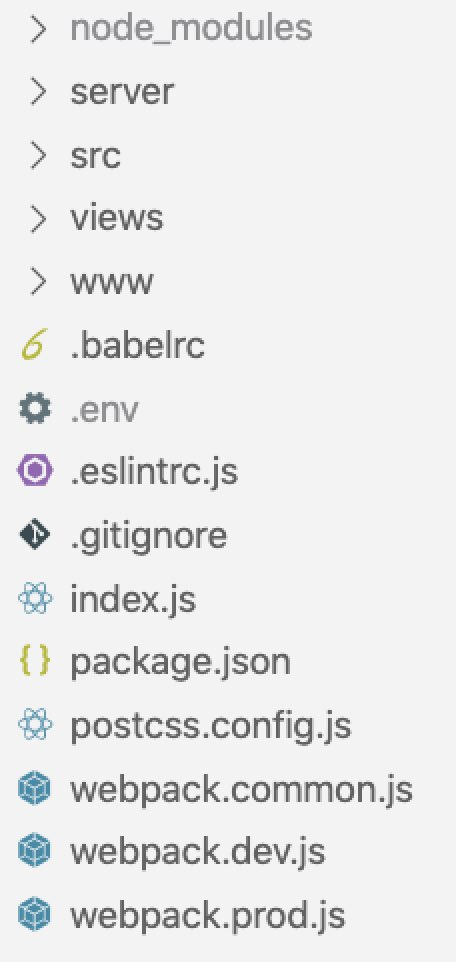
\includegraphics[width=0.3\textwidth]{app}
  \caption{Vista general de la raíz del proyecto.}
\end{figure}

\newpage
\subsubsection{Variables del entorno}
El acceso a las variables de entorno en Node.js es compatible desde el primer momento. Cuando el proceso Node.js se inicia, automáticamente proporciona acceso a todas las variables de entorno existentes al crear un objeto env como propiedad del objeto global del proceso.
\vspace{0.8cm}

\lstinputlisting[style=ES6, caption=Variables principales del sistema]{code/env.txt}


\newpage
\section{Configuración del servidor (Backend)}
Si alguna vez ha utilizado PHP o ASP, probablemente esté acostumbrado a la idea de que el servidor web (Apache o IIS, por ejemplo) sirve sus archivos estáticos para que un navegador puede verlos a través de la red. Node ofrece un paradigma diferente al de un servidor web tradicional: la aplicación es el servidor web. Node simplemente proporciona las bases para que se pueda construir un servidor web. 

\subsection{Servidor NodeJS}
El modelo de E/S impulsado por eventos sin bloqueo le brinda a NodeJS un rendimiento muy atractivo, superando fácilmente los entornos de servidores como PHP y Ruby on Rails, que bloquean las E/S y manejan múltiples usuarios simultáneos en hilos separados para cada uno. Algo importante que se debe saber es que NodeJS no es un \gls{framework} sino un entorno, hay \glspl{framework} que funcionan con Node, como Express y Sails, lo que facilita la creación de aplicaciones.
\vspace{0.8cm}

\begin{figure}[H]
  \centering
  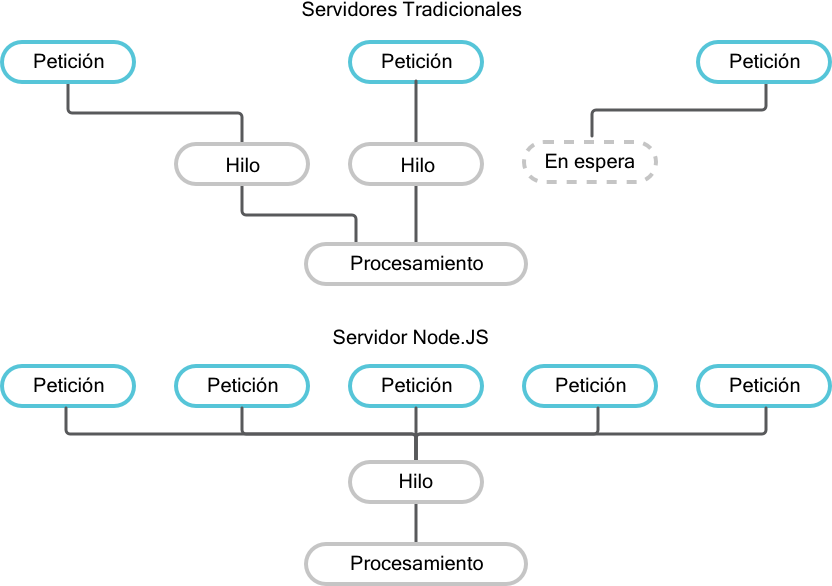
\includegraphics[width=0.8\textwidth]{node-traditional}
  \caption{Comparación de node y servidores tradicionales.}
\end{figure}

Un servidor Node.js tiene un solo subproceso de bucle de eventos (event-loop) que espera E/S en sockets y archivos. Una vez que los datos están listos, activa el método de evento correspondiente y espera hasta que regrese antes de esperar nuevamente por más eventos de E/S. Dado que todas las operaciones de E/S no bloquean, se asegurará de que todo se ejecute correctamente tan pronto como la entrada esté disponible sin ningún bloqueo y sin que se tenga lidiar con problemas de subprocesos múltiples.

\newpage
\subsubsection{Programación basada en eventos}
La filosofía central detrás de NodeJS es la programación basada en eventos. Significa que, el programador,  debe comprender qué eventos están disponibles y cómo responder a ellos. Muchas personas se introducen en la programación basada en eventos mediante la implementación de una interfaz de usuario: el usuario hace clic en algo y se dispara el `evento clic'. Es una buena metáfora, porque se entiende que el programador no tiene control sobre cuándo, o si el usuario va a hacer clic en algo, por lo que la programación basada en eventos es realmente bastante intuitiva \cite{ethan}.
\vspace{0.8cm}

\lstinputlisting[label={node-server}, style=ES6, caption=Configuración servidor NodeJS básico]{code/node-server.js}
En el ejemplo de código \ref{node-server}, el evento es implícito: el evento que se está manejando es una solicitud HTTP. El método http.createServer toma una función como argumento; esta función se invocará cada vez que se realice una solicitud HTTP. El programa simplemente establece el tipo de contenido en texto sin formato y envía la cadena `Hola, mundo!'.


\subsection{Configuración Express}
Express.js es un `marco de aplicación web NodeJS minimalista y flexible' \cite{express}. Es una capa delgada de características, fundamental para cualquier aplicación web, agrega tres características poderosas: enrutamiento, mejores manejadores de solicitudes y vistas.

\subsubsection{Enrutamiento}
Enrutamiento se refiere al mecanismo para servir al cliente el contenido que ha solicitado. Para las aplicaciones cliente/servidor basadas en web, el cliente especifica el contenido deseado en la URL (ruta y cadena de consulta).\\[0.8cm]
Cuando una aplicación Express.js se está ejecutando, escucha las solicitudes. Cada solicitud entrante se procesa de acuerdo con una cadena definida de middlewares y rutas que comienzan de arriba a abajo. Este aspecto es importante porque le permite controlar el flujo de ejecución \cite{azat}.
\vspace{0.8cm}

\begin{figure}[H]
  \centering
  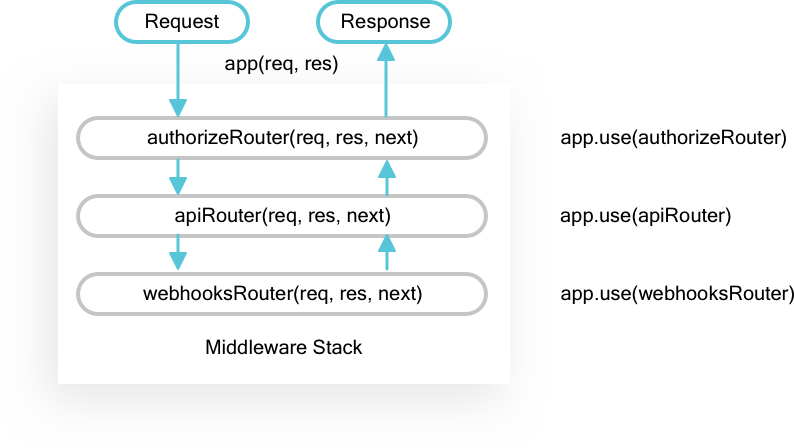
\includegraphics[width=0.8\textwidth]{express-router}
  \caption{Cada función de middleware en la pila se ejecuta antes que las que están debajo de ella. (Fuente: Elaboración propia)}
\end{figure}

\newpage
\lstinputlisting[style=ES6, caption=Fragmento de la configuración de enrutamiento del sistema]{code/express-router.js}

\subsection{Configuración Firebase}
Antes de conectar nuestro sistema con una base de datos de Firestore es necesario crear una aplicación en la consola de Google Firebase y seguir los siguientes pasos.
\vspace{0.8cm}

\begin{figure}[H]
  \centering
  
\includegraphics[width=1\textwidth]{firebase-01}
  \caption{Consola de Google Firebase.}
\end{figure}

\begin{enumerate}
  \item Crear un nuevo proyecto en la consola de Firebase.

  \begin{figure}[H]
    \centering
    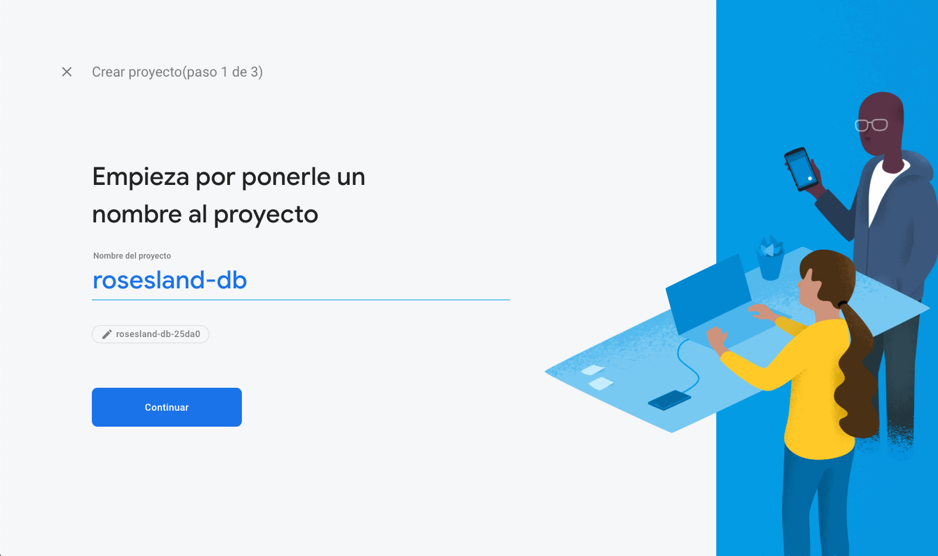
\includegraphics[width=1\textwidth]{firebase-02}
  \end{figure}

  \item En el apartado `Database', seleccionar `crear base de datos' .

  \begin{figure}[H]
    \centering
    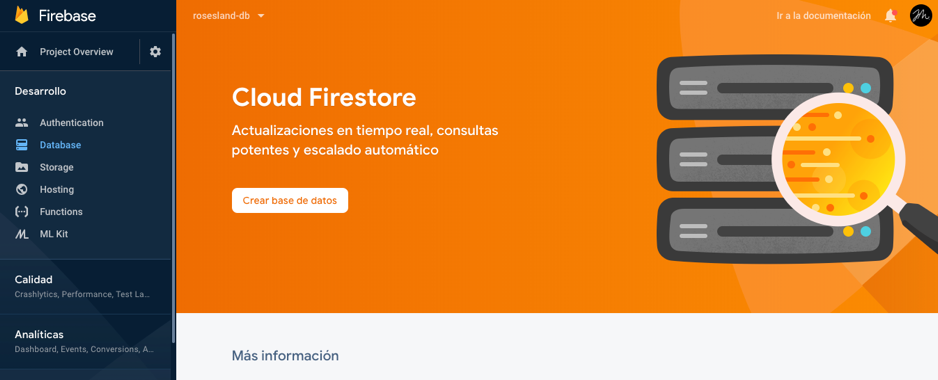
\includegraphics[width=1\textwidth]{firebase-03}
  \end{figure}

  \item En la ventana emergente, seleccionar reglas de seguridad y definir ubicación del servidor.

  \begin{figure}[H]
    \centering
    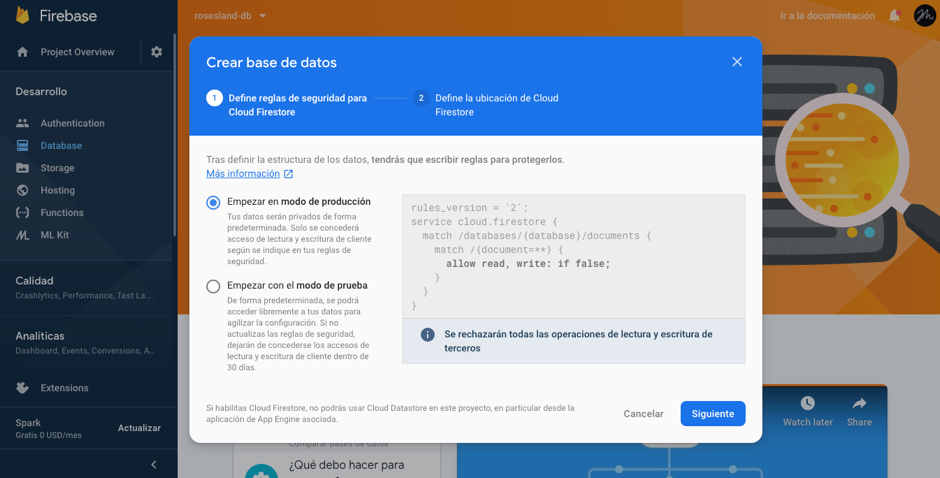
\includegraphics[width=1\textwidth]{firebase-04}
  \end{figure}

  \item El siguiente paso es generar las claves que permitan usar `firebase-admin' en el \textit{backend}. En la configuración del proyecto debajo del apartado `cuentas de servicio', presionar el botón `Generar cuentas de servicio'. El contenido del archivo JSON generado se debe de agregar a las variables del entorno que correspondan.

  \begin{figure}[H]
    \centering
    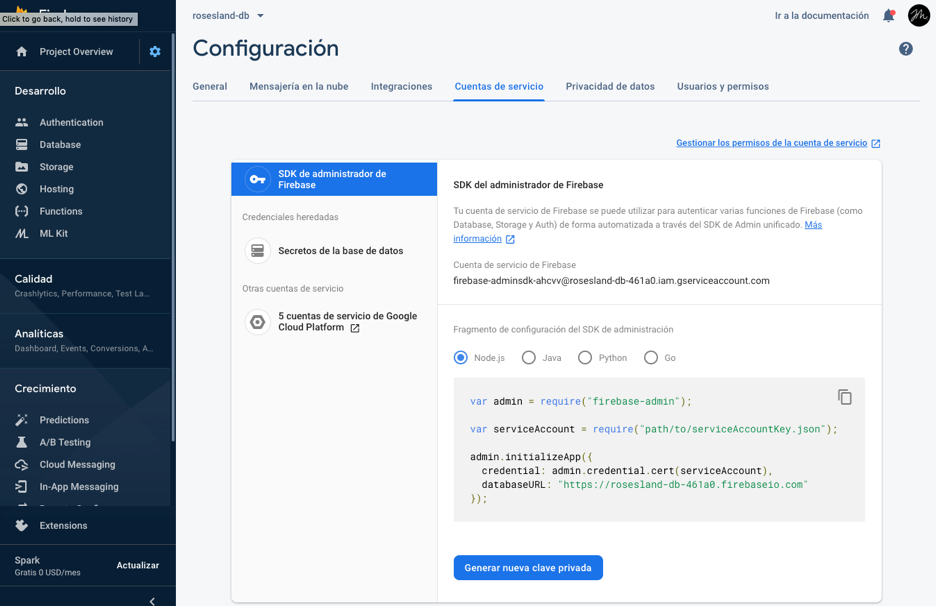
\includegraphics[width=1\textwidth]{firebase-05}
  \end{figure}

  \item Por ultimo en la sección `Authentication' se deben activar los servicios de autenticación necesarios, para este proyecto es necesario activar la validación por correo electrónico y contraseña.

  \begin{figure}[H]
    \centering
    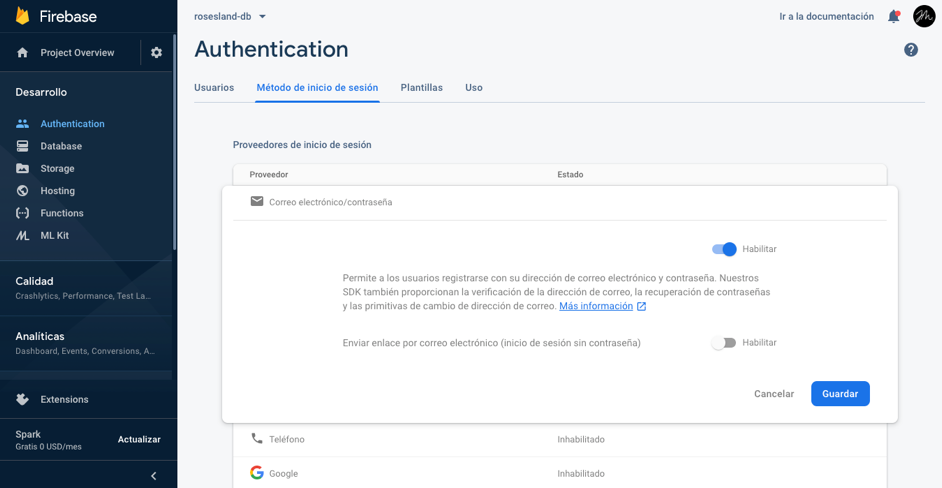
\includegraphics[width=1\textwidth]{firebase-06}
  \end{figure}
\end{enumerate}

\newpage
\subsubsection{Configuración de Firebase Firestore en Node.js}
Después de crear el objeto de configuración, es necesario inicializar Firebase en la aplicación de la siguiente manera:
\vspace{0.8cm}

\lstinputlisting[label={node-firebase}, style=ES6, caption=Fragmento de la configuración Firebase en el servidor]{code/firebase.js}

\subsubsection{Escrituras en lotes}
Para manipular documentos en un conjunto de operaciones, se pueden ejecutar varias operaciones de escritura como un lote único que incluya cualquier combinación de operaciones set(), update() o delete(). El lote de escrituras se completa de forma atómica y puede escribir en varios documentos. Los siguientes ejemplos muestran cómo crear y confirmar un lote de escrituras \cite{transactions}:
\vspace{0.8cm}

\lstinputlisting[label={firebase-function}, style=ES6, caption=Fragmento para guardar datos en Firestore]{code/firebase-function.js}


\subsection{Autenticación}
Casi todas las aplicaciones requieren algún sistema de autorización. En algunos casos, validar un nombre de usuario/contraseña establecido con nuestra tabla de Usuarios es suficiente, pero a menudo, necesitamos un modelo de permisos más detallado para permitir que ciertos usuarios accedan a ciertos recursos y los restrinjan de otros. Construir un sistema para soportar esto último no es trivial y puede llevar mucho tiempo. El API de autenticación basada en roles de Firebase, ayuda a poner todo en marcha rápidamente.

\subsubsection{Autenticación basada en roles}
En este modelo de autorización, se otorga acceso a roles, en lugar de usuarios específicos, y un usuario puede tener uno o más, según cómo diseñe su modelo de permiso. Los recursos, por otro lado, requieren ciertos roles para permitir que un usuario los ejecute.
\vspace{0.8cm}

\begin{figure}[H]
  \centering
  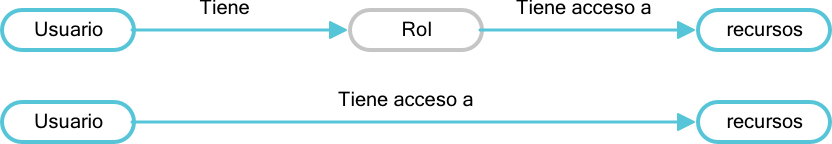
\includegraphics[width=1\textwidth]{firebase-auth}
  \caption{Autenticación basada en roles.}
\end{figure}

\subsubsection{Firebase Custom Claims}
Los roles de usuario son necesarios para identificar a los usuarios como administradores, gerentes o simplemente como clientes. Firebase Custom Claims permite establecer atributos de usuario simples directamente en el JWT del usuario (por ejemplo: \{ admin: true \}). Un JWT es un Json Web Token, es el objeto que contiene la información del usuario actual.
\vspace{0.8cm}

\lstinputlisting[label={firebase-auth}, style=ES6, caption=Fragmento para guardar crear y leer Firebase Custom Claims]{code/firebase-auth.js}

\subsection{Integración con Shopify}
La API de Storefront de Shopify brinda el control creativo completo para crear experiencias de compra personalizadas; se centra en las experiencias de compra vistas desde la perspectiva del cliente. Las características principales del API Storefront son \cite{storefront}:
\begin{itemize}
  \item Obtener datos sobre un solo producto o una colección de productos para mostrar en cualquier sitio web o dispositivo.
  \item Crear experiencias de pago únicas con control total sobre el carrito de compras.
  \item Crear nuevos clientes o modifique los existentes, incluida la información de la dirección.
\end{itemize}
Los motivos aquí son bastantes simples. Se requiere que los usuarios puedan navegar, buscar y seleccionar productos directamente en un dominio personalizado sin tener que ir a la tienda en linea de Shopify.
\vspace{0.8cm}

Una vez realizada una conexión exitosa con la API Storefront de Shopify, es posible crear componentes ReactJS para visualizar imágenes de productos, variaciones de productos, tamaños de productos, etcétera. De este modo el sistema podrá extender el uso de la plataforma.

\newpage
\lstinputlisting[label={node-shopify}, style=ES6, caption=Fragmento de código para la conexión con Shopify]{code/shopify.js}

\subsection{Webhooks}
Un webhook permite que servicios de terceros envíen actualizaciones en tiempo real a su aplicación. Las actualizaciones se activan por algún evento o acción por parte del proveedor de webhook, y se envían a su aplicación a través de solicitudes HTTP. Cuando recibe la solicitud, la maneja con una lógica personalizada, como enviar un correo electrónico o almacenar los datos en una base de datos.

\subsection{Webhooks Shopify}
Un webhook se puede usar para recibir notificaciones sobre eventos particulares en una tienda en linea. Después de suscribirse a un webhook, puede permitir que su aplicación ejecute código inmediatamente después de que ocurran eventos específicos en las tiendas que tienen su aplicación instalada, en lugar de tener que hacer llamadas \acrshort{api} periódicamente para verificar su estado. Por ejemplo, puede configurar un webhook para activar una acción en su aplicación cuando un cliente crea un carrito de compras o cuando un comerciante cree un nuevo producto en su administrador de Shopify. Al usar las suscripciones de webhooks, puede hacer menos llamadas \acrshort{api} en general, lo que garantiza que la aplicación sea más eficiente y se actualice rápidamente \cite{webhook}.
\vspace{0.8cm}

\begin{figure}[H]
  \centering
  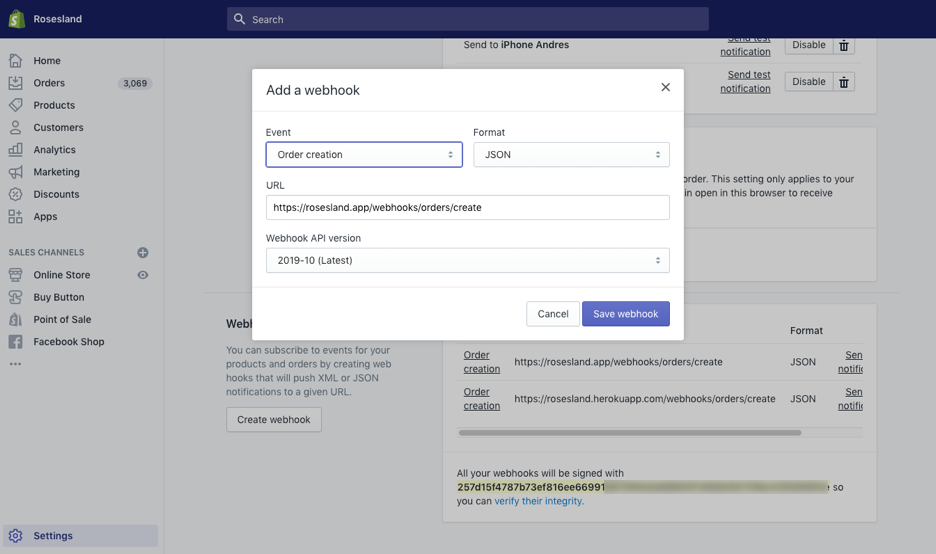
\includegraphics[width=1\textwidth]{webhook}
  \caption{Panel para crear webhooks en Shopify. (Fuente: Shopify Admin)}
\end{figure}

Después de configurar una suscripción de webhook, los eventos que especificó activarán una notificación de webhook cada vez que ocurran. Esta notificación contiene información JSON y encabezados HTTP que proporcionan contexto.

\newpage
\subsection{Configuración de webhook en Express.js}
En lugar de extraer información a través del \acrshort{api}, los webhooks enviarán información a su punto final.
\vspace{0.8cm}

\lstinputlisting[style=ES6, caption=Ruta que capta el webhook lanzado desde Shopify]{code/webhook.js}

\subsection{Websockets con Socket.IO}
Si bien la base de datos Firebase Firestore proporciona una capa de conexión en tiempo real, es necesario introducir un nuevo método de comunicación permanente para notificar de eventos como lo son la presencia de usuarios activos y la visualización de las ordenes. Socket.IO permite la comunicación bidireccional entre el cliente y el servidor. Las comunicaciones bidireccionales se habilitan cuando un cliente tiene Socket.IO en el navegador, y un servidor también ha integrado el paquete. Si bien los datos se pueden enviar de varias formas, JSON es el más simple. Resume muchos tipos de transportes, incluidos AJAX y WebSockets, en una sola API. Permite a los desarrolladores enviar y recibir datos sin preocuparse por la compatibilidad entre navegadores \cite{kelleher}.
\vspace{0.8cm}

En cualquier aplicación en tiempo real, mostrar múltiples usuarios en línea es muy importante, esta información debe actualizarse cuando un nuevo usuario se conecta o un usuario en línea se desconecta.
\vspace{0.8cm}

\lstinputlisting[style=ES6, caption=Fragmento de configuración de Socket.IO del sistema]{code/socket.js}

\newpage
\section{Patrones de diseño}
Los patrones de diseño facilitan la reutilización de diseños y arquitecturas exitosas. Los patrones de diseño ayudan a elegir alternativas de diseño que hacen que un sistema sea reutilizable y evitar alternativas que comprometan la reutilización. Pueden incluso mejorar la documentación y el mantenimiento de los sistemas existentes.
\subsection{Redux}
Redux es un administrador de estado predecible para aplicaciones JavaScript basado en el patrón de diseño Flux. A medida que una aplicación crece, se hace difícil mantenerla organizada y mantener el flujo de datos. Redux resuelve este problema administrando el estado de la aplicación con un único objeto global llamado Store. Los principios fundamentales de Redux ayudan a mantener la coherencia en toda la aplicación, lo que facilita la depuración y las pruebas.
\subsubsection{Redux Store}
Redux Store contiene un objeto del estado global de la aplicación. Esta actualiza el estado y notifica los componentes suscritos. \\[0.8cm]
\lstinputlisting[style=ES6, caption=Fragmento de código para inicializar el Store]{code/redux-store.js}

\subsubsection{Redux Reducer}
Un Reducer es solo una función pura de JavaScript. Recibe dos parámetros: el estado actual y la acción. Una función pura es aquella que devuelve exactamente la misma salida para la entrada dada. El estado es el objeto Store completo, la acción es el objeto despachado con un tipo requerido y un payload opcional. \\[0.8cm]
\lstinputlisting[style=ES6, caption=Fragmento de código del reducer común de la app]{code/redux-reducer.js}

\subsubsection{Acciones Redux}
La única forma de cambiar el estado es enviando una señal a el Store. Esta señal es una acción. Entonces "despachar una acción" significa enviar una señal a el Store. \\[0.8cm]
\lstinputlisting[style=ES6, caption=Fragmento de código de la acción que valida a un administrador]{code/redux-action.js}


\newpage
\section{Integración React/Redux}
Para conectar el Store de Redux con React, es mediante un componente llamado Provider. El único propósito de Provider es agregar el Store al contexto del componente de la Aplicación, para que todos los componentes secundarios puedan acceder a ella. Provider envuelve a la aplicación React y hace que sea consciente de el Store. \\[0.8cm]
\lstinputlisting[style=ES6, caption=Fragmento de código de la aplicación React principal]{code/redux-react.js}



\section{Requerimientos del proyecto}
El producto final está enfocado en incrementar las ventas de la empresa Rosesland, con la ayuda de una plataforma que administre y mejore sus procesos internos. La finalidad del proyecto es disminuir los tiempos de ventas, elaboración y entrega de productos, así como la de crear un vínculo entre el servidor y su infraestructura actual extendiendo sus capacidades.
\vspace{0.8cm}

El sistema debe adaptarse al sistema operativo Linux. Anticipado a futuros cambios en la plataforma se decide trabajar con Node.js, ya que es de código abierto y multiplataforma, esto permite beneficiarse de la reutilización del código y la falta de cambio de contexto. Las aplicaciones Node.js están escritas en JavaScript puro y pueden ejecutarse dentro del entorno Node.js en Windows, Linux, etc.
\vspace{0.8cm}

La interfaz gráfica de usuario de la aplicación debe ser responsiva y funcionar en la mayoría de los navegadores web modernos, además debe ser fácil de aprender, idealmente requerir poco entrenamiento.
\vspace{0.8cm}

\subsection{Herramientas}
Node.js permite incorporar herramientas poderosas a proyectos de cualquier tipo. Esto incluye todo, desde bibliotecas y \glspl{framework} como jQuery y AngularJS hasta procesadores de código como Webpack. Los paquetes vendrán en una carpeta típicamente llamada node\_modules, que también contendrá un archivo package.json. Este archivo contiene información sobre todos los paquetes, incluidas las dependencias, que son módulos adicionales necesarios para usar un paquete en particular.

\subsubsection{Dependencias de desarrollo}
Las dependencias de desarrollo son aquellas que se utilizan dentro del entorno de programación. Aquí se incluyen herramientas que no forman parte del ejecutable final como lo son lo preprocesadores, empaquetadores y analistas de código. Los principales módulos de desarrollo son los siguientes:
\begin{itemize}
  \item Babel: es un compilador de JavaScript utilizado para convertir código ECMAScript 2015+ (ES6+) en una versión que pueda ser ejecutado en motores JavaScript más antiguos.
  \item Webpack: es un empaquetador de módulos principalmente para JavaScript, pero puede transformar archivos \gls{frontend} como HTML, CSS e imágenes si se incluyen los complementos correspondientes.
  \item ESLint: es una herramienta de análisis de código estático para identificar patrones problemáticos encontrados en el código JavaScript.
  \item PostCSS: es una herramienta de desarrollo de software que utiliza complementos basados en JavaScript para automatizar las operaciones de rutina de CSS. Con este modulo es posible analizar CSS, agregar prefijos de proveedor a las reglas CSS, ejecutar optimizaciones enfocadas, para garantizar que el resultado final sea lo más pequeño posible para un entorno de producción.
  \item Pug: es un preprocesador que simplifica la tarea de escribir HTML. También agrega funcionalidades, como objetos Javascript, condiciones, bucles, \glspl{mixin} y plantillas.
\end{itemize}

\subsubsection{Estructura del proyecto}
La estructura del proyecto Node.js está influenciada por preferencias personales, la arquitectura del proyecto y la estrategia de inyección de módulos que se está utilizando. Para tener una estructura FERN, es imperativo separar el código fuente del servidor y el utilizado por el cliente, ya que el código del lado del cliente o \gls{frontend} probablemente se minimizará y se enviará al navegador y es público en su naturaleza básica. Y el lado del servidor o el \gls{backend} proporcionarán \acrshort{api} para realizar operaciones \acrshort{crud}.

\subsubsection{Directorios}
\begin{itemize}
  \item node\_modules: Directorio oculto que contiene las dependencias generales del proyecto, este archivo debe ser ignorado por el controlador de versiones.
  \item server: Aquí se encuentran los archivos requeridos por el servidor para el enrutamiento, la conexión con la base de datos y las funciones de utilidad del \gls{backend}.
  \item src: Este directorio concentra todos los elementos necesarios para producir nuestra aplicación cliente.
  \item views: En esta carpeta se incluyen los templates necesarios para generar las vistas HTML de nuestro proyecto.
  \item www: Su propósito es contener los archivos del cliente, aquí podemos encontrar el código de producción de nuestra aplicación web compilado y minificado, así como las hojas de estilo, imágenes, fuentes tipográficas, vectores, etc.
\end{itemize}

\subsubsection{Archivos principales}
\begin{itemize}
  \item .babelrc: Contiene los mecanismos necesarios para compilar sintaxis moderna de JavaScript y una lista con los navegadores web a los que se requiere dar enfoque.
  \item .env: Documento oculto que contiene las variables del entorno, este archivo es ignorado por el controlador de versiones.
  \item .eslintrc.js: En este archivo se declaran las reglas para identificar e informar sobre patrones o errores encontrados en el código.
  \item .gitignore: Aquí se describen los archivos y directorios que deben ser ignorados por Git.
  \item index.js: Entrada principal de nuestro servidor, contiene el código necesario para que el proyecto funcione correctamente.
  \item package.json: Este archivo puede contener muchos metadatos sobre su proyecto. Pero principalmente se usa para dos cosas:
  \begin{itemize}
    \item Gestionar dependencias de su proyecto
    \item Scripts, que ayudan a generar compilaciones, ejecutar pruebas y otras cosas con respecto al proyecto
  \end{itemize}
\end{itemize}

\begin{figure}[H]
  \centering
  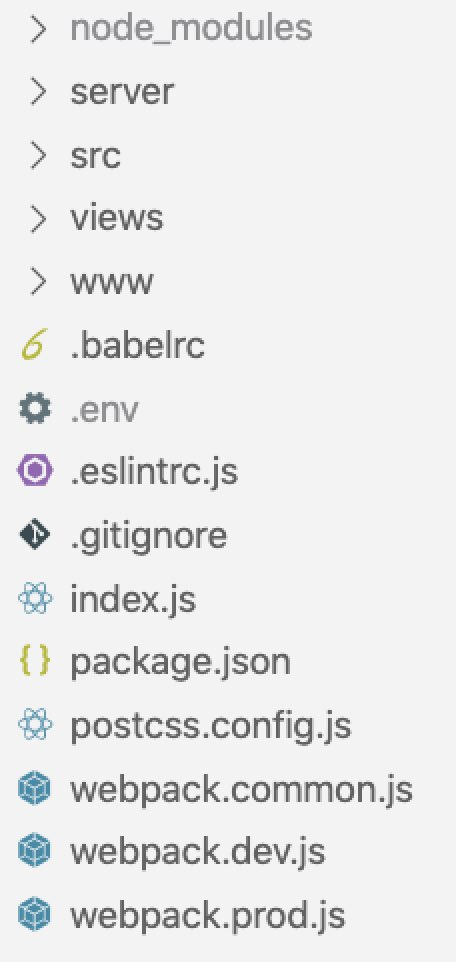
\includegraphics[width=0.3\textwidth]{app}
  \caption{Vista general de la raíz del proyecto.}
\end{figure}

\newpage
\subsubsection{Variables del entorno}
El acceso a las variables de entorno en Node.js es compatible desde el primer momento. Cuando el proceso Node.js se inicia, automáticamente proporciona acceso a todas las variables de entorno existentes al crear un objeto env como propiedad del objeto global del proceso.
\vspace{0.8cm}

\lstinputlisting[style=ES6, caption=Variables principales del sistema]{code/env.txt}


\newpage
\section{Patrón de diseño}
Los patrones de diseño facilitan la reutilización de diseños y arquitecturas exitosas. Los patrones de diseño ayudan a elegir alternativas de diseño que hacen que un sistema sea reutilizable y evitar alternativas que comprometan la reutilización. Pueden incluso mejorar la documentación y el mantenimiento de los sistemas existentes.
\subsection{Redux}
Redux es un administrador de estado predecible para aplicaciones JavaScript basado en el patrón de diseño Flux. A medida que una aplicación crece, se hace difícil mantenerla organizada y mantener el flujo de datos. Redux resuelve este problema administrando el estado de la aplicación con un único objeto global llamado Store. Los principios fundamentales de Redux ayudan a mantener la coherencia en toda la aplicación, lo que facilita la depuración y las pruebas.
\subsubsection{Redux Store}
Redux Store contiene un objeto del estado global de la aplicación. Esta actualiza el estado y notifica los componentes suscritos. \\[0.8cm]
\lstinputlisting[style=ES6, caption=Fragmento de código para inicializar el Store]{code/redux-store.js}

\subsubsection{Redux Reducer}
Un Reducer es solo una función pura de JavaScript. Recibe dos parámetros: el estado actual y la acción. Una función pura es aquella que devuelve exactamente la misma salida para la entrada dada. El estado es el objeto Store completo, la acción es el objeto despachado con un tipo requerido y un payload opcional. \\[0.8cm]
\lstinputlisting[style=ES6, caption=Fragmento de código del reducer común de la app]{code/redux-reducer.js}

\subsubsection{Acciones Redux}
La única forma de cambiar el estado es enviando una señal a el Store. Esta señal es una acción. Entonces "despachar una acción" significa enviar una señal a el Store. \\[0.8cm]
\lstinputlisting[style=ES6, caption=Fragmento de código de la acción que valida a un administrador]{code/redux-action.js}


\newpage
\section{Integración React/Redux}
Para conectar el Store de Redux con React, es mediante un componente llamado Provider. El único propósito de Provider es agregar el Store al contexto del componente de la Aplicación, para que todos los componentes secundarios puedan acceder a ella. Provider envuelve a la aplicación React y hace que sea consciente de el Store. \\[0.8cm]
\lstinputlisting[style=ES6, caption=Fragmento de código de la aplicación React principal]{code/redux-react.js}


\newpage
\section{E-commerce (Comercio electrónico)}
El comercio electrónico se refiere al proceso de compra o venta de productos o servicios a través de Internet. 
Las compras en línea se están volviendo cada vez más populares debido a la velocidad y facilidad de uso para los clientes. 
Las actividades de comercio electrónico, como la venta en línea, pueden dirigirse a consumidores u otras empresas. 
% Business to Consumer (B2C) implica la venta en línea de bienes, servicios y el suministro de información directamente a los consumidores. 
% Business to Business (B2B) se refiere al intercambio en línea de productos, servicios o información entre empresas.
Vender en línea puede ayudar a su empresa a llegar a nuevos mercados y aumentar sus ventas e ingresos 
(ya sea a través de su propio sitio web o de un sitio de mercado electrónico).
\subsubsection{Shopify}
Shopify es un servicio web que le permite configurar una tienda en línea para vender sus productos. 
Le da la facilidad organizar sus productos, personalizar el diseño de su tienda, 
aceptar pagos con tarjeta de crédito, rastrear y responder a pedidos. 
Shopify.com permite a los vendedores elegir entre opciones de diseño gratuitas 
o diseños personalizados creados por los usuarios.

\end{document}